% \iffalse meta-comment
%
% Copyright (C) 2018--2023 by Xiangdong Zeng <xdzeng96@gmail.com>
%
% This work may be distributed and/or modified under the
% conditions of the LaTeX Project Public License, either
% version 1.3c of this license or (at your option) any later
% version. The latest version of this license is in:
%
%   http://www.latex-project.org/lppl.txt
%
% and version 1.3 or later is part of all distributions of
% LaTeX version 2005/12/01 or later.
%
% This work has the LPPL maintenance status `maintained'.
%
% The Current Maintainer of this work is Xiangdong Zeng.
%
% \fi

%*********************************************************************
% fduthesis: 复旦大学论文模板
% 2023-05-27 v0.9a
%
% 重要提示：
%   1. 请确保使用 UTF-8 编码保存
%   2. 请使用 XeLaTeX 或 LuaLaTeX 编译
%   3. 请仔细阅读用户文档
%   4. 修改、使用、发布本文档请务必遵循 LaTeX Project Public License
%   5. 不需要的注释可以尽情删除
%*********************************************************************

\documentclass[type=master]{fduthesis}
% 模板选项：
%   type = doctor|master|bachelor  论文类型，默认为本科论文
%   oneside|twoside                论文的单双面模式，默认为 twoside
%   draft = true|false             是否开启草稿模式，默认关闭
% 带选项的用法示例：
%   \documentclass[oneside]{fduthesis}
%   \documentclass[twoside, draft=true]{fduthesis}
%   \documentclass[type=bachelor, twoside, draft=true]{fduthesis}

\fdusetup{
  % 参数设置
  % 允许采用两种方式设置选项：
  %   1. style/... = ...
  %   2. style = { ... = ... }
  % 注意事项：
  %   1. 不要出现空行
  %   2. “=” 两侧的空格会被忽略
  %   3. “/” 两侧的空格不会被忽略
  %   4. 请使用英文逗号 “,” 分隔选项
  %
  % style 类用于设置论文格式
  style = {
    % font = times,
    % 西文字体（包括数学字体）
    % 允许选项：
    %   font = garamond|libertinus|lm|palatino|times|times*|none
    %
    % cjk-font = fandol,
    % 中文字体
    % 允许选项：
    %   cjk-font = adobe|fandol|founder|mac|sinotype|sourcehan|windows|none
    %
    % 注意：
    %   1. 中文字体设置高度依赖于系统。各系统建议方案：
    %        windows：cjk-font = windows
    %        mac：    cjk-font = mac
    %        linux：  cjk-font = fandol（默认值）
    %   2. 除 fandol 和 sourcehan 外，其余字体均为商用字体，请注意版权问题
    %   3. 但 fandol 字体缺字比较严重，而 sourcehan 没有配备楷体和仿宋体
    %   4. 这里中西文字体设置均注释掉了，即使用默认设置：
    %        font     = times
    %        cjk-font = fandol
    %   5. 使用 font = none / cjk-font = none 关闭默认字体设置，需手动进行配置
    %
    % font-size = -4,
    % 字号
    % 允许选项：
    %   font-size = -4|5
    %
    % fullwidth-stop = catcode,
    % 是否把全角实心句点 “．” 作为默认的句号形状
    % 允许选项：
    %   fullwidth-stop = catcode|mapping|false
    % 说明：
    %   catcode   显式的 “。” 会被替换为 “．”（e.g. 不包括用宏定义保存的 “。”）
    %   mapping   所有的 “。” 会被替换为 “．”（使用 LuaLaTeX 编译则无效）
    %   false     不进行替换
    %
    footnote-style = xits,
    % 脚注编号样式
    % 允许选项：
    %   footnote-style = plain|libertinus|libertinus*|libertinus-sans|
    %                    pifont|pifont*|pifont-sans|pifont-sans*|
    %                    xits|xits-sans|xits-sans*
    % 默认与西文字体保持一致
    %
    % hyperlink = color,
    % 超链接样式
    % 允许选项：
    %   hyperlink = border|color|none
    %
    % hyperlink-color = default,
    % 超链接颜色
    % 允许选项：
    %   hyperlink-color = default|classic|material|graylevel|prl
    %
    bib-backend = bibtex,
    % 参考文献支持方式
    % 允许选项：
    %   bib-backend = bibtex|biblatex
    %
    % bib-style = numerical,
    % 参考文献样式
    % 允许选项：
    %   bib-style = author-year|numerical|<其他样式>
    % 说明：
    %   author-year  著者—出版年制
    %   numerical    顺序编码制
    %   <其他样式>   使用其他 .bst（bibtex）或 .bbx（biblatex）格式文件
    %
    % cite-style = {},
    % 引用样式
    % 默认为空，即与参考文献样式保持一致
    % 仅适用于 biblatex；如要填写，需保证相应的 .cbx 格式文件能被调用
    %
    bib-resource = {main.bib},
    % 参考文献数据源
    % 可以是单个文件，也可以是用英文逗号 “,” 隔开的一组文件
    % 如果使用 biblatex，则必须明确给出 .bib 后缀名
    %
    % logo = {fudan-name.pdf},
    % 封面中的校名图片
    % 模版已自带，通常不需要额外配置
    %
    % logo-size = {0.5\textwidth},      % 只设置宽度
    % logo-size = {{}, 3cm},            % 只设置高度
    % logo-size = {8cm, 3cm},           % 设置宽度和高度
    % 设置校名图片的大小
    % 通常不需要调整
    %
    % declaration-page = {declaration.pdf},
    % 插入扫描版的声明页 PDF 文档
    % 默认使用预定义的声明页，但不带签名
    %
    % auto-make-cover = true
    % 是否自动生成论文封面（封一）、指导小组成员名单（封二）和声明页（封三）
    % 除非特殊需要（e.g. 不要封面），否则不建议设为 false
  },
  %
  % info 类用于录入论文信息
  info = {
    title = {低温晶体量热器系统减振研究},
    % 中文标题
    % 长标题建议使用 “\\” 命令手动换行（不是指在源文件里输入回车符，当然
    % 源文件里适当的换行可以有助于代码清晰）：
    %   title = {最高人民法院、最高人民检察院关于适用\\
    %            犯罪嫌疑人、被告人逃匿、死亡案件违法所得\\
    %            没收程序若干问题的规定},
    %
    title* = {Vibration Reduction Research for Bolometer Systems},
    % 英文标题
    %
    author = {曹华琦},
    % 作者姓名
    %
    % author* = {Your name},
    % 作者姓名（英文 / 拼音）
    % 目前不需要填写
    %
    supervisor = {马龙\quad 青年研究员},
    % 导师
    % 姓名与职称之间可以用 \quad 打印一个空格
    %
    major = {粒子物理与原子核物理},
    % 专业
    %
    degree = academic,
    % 学位类型
    % 允许选项：
    %   degree = academic|professional
    % 说明：
    %   academic      学术学位
    %   professional  专业学位
    %
    department = {物理系},
    % 院系
    %
    student-id = {24210200001},
    % 作者学号
    %
    % date = {2023 年 1 月 1 日},
    % 日期
    % 注释掉表示使用编译日期
    %
    % secret-level = ii,
    % 密级
    % 允许选项：
    %   secret-level = none|i|ii|iii
    % 说明：
    %   none  不显示密级与保密年限
    %   i     秘密
    %   ii    机密
    %   iii   绝密
    %
    % secret-year = {五年},
    % 保密年限
    % secret-level = none 时该选项无效
    %
    instructors = {
      {陈\quad 昊 \quad 教\quad 授},
      {黄\quad 焕 \quad 中\quad 教\quad 授},
    },
    % 指导小组成员
    % 使用英文逗号 “,” 分隔
    % 如有需要，可以用 \quad 手工对齐
    %
    keywords = {振动；脉冲管制冷机；低温晶体量热器},
    % 中文关键词
    % 使用英文逗号 “,” 分隔
    %
    keywords* = {Vibration; Pulse tube cryocooler; Bolometer},
    % 英文关键词
    % 使用英文逗号 “,” 分隔
    %
    clc = {O413.1},
    % 中图分类号
    %
    % jel = {C02},
    % JEL 分类号，仅适用于经济学院等部分院系
  }
}

% 需要的宏包可以自行调用
\usepackage{physics}

% 需要的命令可以自行定义
\newcommand{\hilbertH}{\symcal{H}}
\newcommand{\ee}{\symrm{e}}
\newcommand{\ii}{\symrm{i}}

\begin{document}

% 这个命令用来关闭版心底部强制对齐，可以减少不必要的 underfull \vbox 提示，但会影响排版效果
% \raggedbottom

% 前置部分包含目录、中英文摘要以及符号表等
\frontmatter

% 目录
\tableofcontents
% 插图目录
\listoffigures
% 表格目录
\listoftables

\begin{abstract}
  中文摘要
\end{abstract}

\begin{abstract*}
  English abstract
\end{abstract*}

% 符号表
% 语法与 LaTeX 表格一致：列用 & 区分，行用 \\ 区分
% 如需修改格式，可以使用可选参数：
%   \begin{notation}[ll]
%     $x$ & 坐标 \\
%     $p$ & 动量
%   \end{notation}
% 可选参数与 LaTeX 标准表格的列格式说明语法一致
% 这里的 “ll” 表示两列均为自动宽度，并且左对齐

% 主体部分是论文的核心
\mainmatter

% 建议采用多文件编译的方式
% 比较好的做法是把每一章放进一个单独的 tex 文件里，并在这里用 \include 导入，例如
%   \include{chapter1}
%   \include{chapter2}
%   \include{chapter3}

\chapter{绪论}

无中微子双贝塔衰变是一种重要的超出标准模型的新物理。在数十年理论和实验的发展与探索的基础上，人们对其可能的物理机制以及实验的技术需求已有较为深刻的理解。国际上有多个实验组通过不同的探测器技术尝试寻找无中微子双贝塔衰变事件，并对半衰期下限给出了$10^{26}$年量级的限制。目前各实验组正在积极进
行下一代实验装置的预研和建设，致力于将半衰期灵敏度提高到$10^{27}$年以上。中国正依托锦屏地下实验室国际领先的实验环境，开发多个不同路线的探测技术。

{\color{red} 以上引自}\cite{Wang2025}。


\section{从贝塔衰变到无中微子双贝塔衰变}

\subsection{贝塔衰变$\beta$}
1896年，贝克勒尔(Becquerel)发现原子核的天然放射性，开启了研究原子核放射性的时代。在天然放射线中的电子射线称为贝塔(β)射线，产生这种射线流的衰变模式称为β衰变。
在对β衰变放射电子进行能谱测量时，发现β能谱为连续谱，不具有阿尔法(α)和伽马( γ)衰变这种二体反应中观察到的分立能峰的特征。基于能量、动量守恒，为解释能谱的“畸变”，泡利
(Pauli)猜想β衰变在放射出电子的同时还发射了一个电中性、质量极低、反应截面很小的粒子，这一粒子带走了一部分能量和动量从而形成了电子的连续谱。1933年，费米(Fermi)将这种粒子改名
为中微子(neutrino)，并且建立了 β 衰变核子流和轻子流相互耦合的有效场论\cite{Fermi1933,Fermi1934a,Fermi1934b}，β 衰变的反应式如下：
\[%beta 衰变反应式
  {}^{A}_{Z}\mathrm{N} \rightarrow {}^{A}_{Z+1}\mathrm{N} + e^{-} + \bar{\nu}_{e} \, .
\]
其中 $e^{-}$ 是 $\beta$ 射线，$\bar{\nu}_{e}$ 是反电子中微子，为 $\beta$ 衰变中发射的中微子类型，轻子数 $L=-1$。电子（$e^{-}$）的轻子数是 $+1$，
因此反应前后的轻子数守恒 $\Delta L = 0$。

{\color{red} 以上引自}\cite{Wang2025}。


\subsection{双贝塔衰变$2\nu\beta\beta$}
1935 年，迈耶（Mayer）基于费米的理论提出，部分偶偶核${}^{A}_{Z}\mathrm{N}$ 由于核子配对效应质量低于 ${}^{A}_{Z+1}\mathrm{N}$，
不能发生 $\beta$ 衰变，但可能出现双贝塔衰变过程（$2\nu\beta\beta$）\cite{Goeppert1935}。
\[
  {}^{A}_{Z}\mathrm{N} \rightarrow {}^{A}_{Z+2}\mathrm{N} + 2e^{-} + 2\bar{\nu}_{e} \, .
\]
$2\nu\beta\beta$ 同样满足轻子数守恒。

{\color{red} 以上引自}\cite{Wang2025}。


\subsection{无中微子双贝塔衰变$0\nu\beta\beta$}
1937 年，马约拉纳（Majorana）指出中微子可能具有反粒子是其本身的马约拉纳属性\cite{Majorana1937}：
\[
  \nu_{e} = \bar{\nu}_{e} \, .
\]

\begin{figure}[htbp]
  \centering
  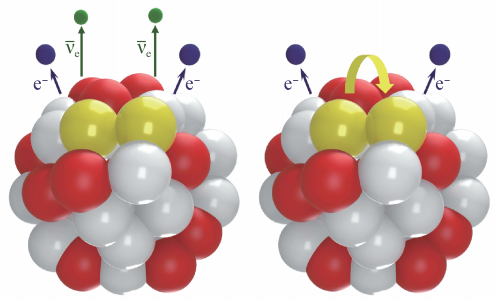
\includegraphics[width=0.75\textwidth]{../figures/double_beta.png}
  \caption{双贝塔衰变过程（2$\nu\beta\beta$，左图）与无中微子双贝塔衰变过程（0$\nu\beta\beta$，右图）示意图}
  \label{fig:double-beta}
\end{figure}

1939 年，弗里（Furry）发现这种中微子的马约拉纳属性可以导致能够发生 $2\nu\beta\beta$ 的核素，也可以发生无中微子双贝塔衰变（$0\nu\beta\beta$）（图~\ref{fig:double-beta} \cite{Wang2025}）\cite{Furry1939}。
\[
  {}^{A}_{Z}\mathrm{N} \rightarrow {}^{A}_{Z+2}\mathrm{N} + 2e^{-} \, .
\]

对于这一反应的物理机制可以简单理解为由于中微子的马约拉纳属性，$2\nu\beta\beta$ 释放的两个中微子发生了湮灭，轻子数不再守恒。1982 年，谢克特（Schechter）和瓦尔（Valle）提出的 Schechter–Valle 定理表明只要 $0\nu\beta\beta$ 发生，则不管反应机制如何，中微子一定具有马约拉纳属性\cite{Schechter1982}。这一理论结果进一步推进了 $0\nu\beta\beta$ 的研究意义。

{\color{red} 以上引自}\cite{Wang2025}。

\section{无中微子双贝塔衰变物理机制简介及实验研究意义}

\subsection{物理机制简介}
对 0νββ 的产生机制有多种不同的理论诠释，本节将介绍目前最为主流简洁的活性感马约拉纳中微子交换机制。

在活性马约拉纳中微子交换机制中，中微子在 SM 中的三种味本征态 
$\nu_e, \nu_\mu, \nu_\tau$ 为三种质量本征态 
$\nu_1, \nu_2, \nu_3$ 的混合，他们的转化关系由一个 3×3 的轻子味混合矩阵 $U$ 表示：

\[
\begin{pmatrix}
\nu_e \\ 
\nu_\mu \\ 
\nu_\tau
\end{pmatrix}
=
\begin{pmatrix}
U_{e1} & U_{e2} & U_{e3} \\
U_{\mu 1} & U_{\mu 2} & U_{\mu 3} \\
U_{\tau 1} & U_{\tau 2} & U_{\tau 3}
\end{pmatrix}
\begin{pmatrix}
\nu_1 \\ 
\nu_2 \\ 
\nu_3
\end{pmatrix},
\tag{5}
\]

0νββ 的半衰期可以用下面的公式表示 \cite{Masaru1981a, Masaru1981b}：

\[
\frac{1}{T_{1/2}^{0\nu}} = G^{0\nu}\left| M^{0\nu} \right|^2
\frac{m_{\beta\beta}^{\,2}}{m_e^{\,2}},
\tag{6}
\]

其中 $T_{1/2}^{0\nu}$ 为对应核素的 0νββ 半衰期；$G^{0\nu}$ 为相空间因子；
$M^{0\nu}$ 为核矩阵元，其计算困难在于如何计算多体问题的初末态原子核波函数；
$m_e$ 为电子质量；$m_{\beta\beta}$ 为中微子的有效质量，其定义为：

\[
m_{\beta\beta} = m_1 U_{e1}^2 + m_2 U_{e2}^2 + m_3 U_{e3}^2.
\tag{7}
\]

在此公式的基础上，可以在中微子振荡实验结果之上估计 $m_{\beta\beta}$ 可能的范围，为实验的发展提供参考。

中微子振荡实验测量了 $U$ 中质量本征态之间的混合角以及质量本征态之间的质量差，但仍存在三个未知特性：(1) 不知道质量本征态之间的质量顺序是正常序 $(m_1 < m_2 < m_3)$ 还是反序 $(m_3 < m_1 < m_2)$；(2) 不知道中微子的绝对质量大小；(3) 
$m_{\beta\beta}$ 理论式中的马约拉纳相位是未知且 0νββ 是其目前唯一可能的测量方式。

{\color{red} 以上引自}\cite{Wang2025}。



\subsection{实验研究意义}




\subsection{研究历程和机遇}
早在20世纪40年代0νββ理论提出不久，相关实验就已经开始进行。随着理论的发展和标准模型（Standard Model，SM）的提出，物理学家们意识到0νββ的发生依赖于中微子的马约拉纳纳属性，而马约拉纳纳属性又意味着中微子存在质量\cite{Schechter1982,
  Racah1937}。这一方面大大提高了对0νββ半衰期的预期，增加了实验难度，另一方面又提升了0νββ的研究意义，使其成为超出标准模型（beyond Standard Model, BSM）新物理机制研究的重要渠道。

0νββ实验研究的另一次转折发生在20世纪末，日本超级神冈实验\cite{Fukuda1998}和加拿大的斯诺（SNO）实验\cite{Ahmad2002}确立了中微子振荡现象，这是人类第一次观测到BSM的物理现象，同时验证了中微子存在质量的本征态。中微子振荡表明中微子存在质量，为其马约拉纳纳属性提供了存在基础，促成了新世纪0νββ实验研究的极大发展。近年来，在欧盟长期科学发展规划\cite{Bracco2017}和美国国家能源部及自然科学基金委核科学长远规划书\cite{Dodge2024}中，0νββ实验均列为优先发展的重大科学实验项目。




\section{低温晶体量热器技术及CUPID-China实验简介}

\subsection{低温晶体量热器技术介绍}




\subsection{CUPID-China实验}




\chapter{干式稀释制冷机中的振动来源与噪声分析}

\section{干式稀释制冷机}

\subsection{脉冲管制冷机(PT)}
\section{其他噪声来源分析}
\subsection{功率密度谱分析}
\section{振动对低温量热器的影响}

\chapter{减振系统设计与搭建}
\section{减振系统设计}
\section{减振系统搭建}
\chapter{减振系统性能测试与分析}

\chapter{总结与展望}

% 附录部分
\appendix

\chapter{公式推导}

% 后置部分包含参考文献、声明页（自动生成）等
\backmatter

% 打印参考文献列表
\printbibliography

\begin{acknowledgements}
  致谢
\end{acknowledgements}

\end{document}
